%%
%% This is file `sample-sigconf.tex',
%% generated with the docstrip utility.
%%
%% The original source files were:
%%
%% samples.dtx  (with options: `sigconf')
%% 
%% IMPORTANT NOTICE:
%% 
%% For the copyright see the source file.
%% 
%% Any modified versions of this file must be renamed
%% with new filenames distinct from sample-sigconf.tex.
%% 
%% For distribution of the original source see the terms
%% for copying and modification in the file samples.dtx.
%% 
%% This generated file may be distributed as long as the
%% original source files, as listed above, are part of the
%% same distribution. (The sources need not necessarily be
%% in the same archive or directory.)
%%
%% The first command in your LaTeX source must be the \documentclass command.
%\documentclass[sigconf]{acmart}
\documentclass[manuscript,screen]{acmart}
%manuscript,screen
\usepackage{multirow}

%%
%% \BibTeX command to typeset BibTeX logo in the docs
\AtBeginDocument{%
  \providecommand\BibTeX{{%
    \normalfont B\kern-0.5em{\scshape i\kern-0.25em b}\kern-0.8em\TeX}}}

%% Rights management information.  This information is sent to you
%% when you complete the rights form.  These commands have SAMPLE
%% values in them; it is your responsibility as an author to replace
%% the commands and values with those provided to you when you
%% complete the rights form.
\setcopyright{acmcopyright}
\copyrightyear{2020}
\acmYear{2020}
\acmDOI{10.1145/1122445.1122456}

%% These commands are for a PROCEEDINGS abstract or paper.
\acmConference[CHI 2021]{CHI 2021: ACM XXXXXX}{May 8--13, 2021}{Yokohama, Japan}
\acmBooktitle{}
\acmPrice{15.00}
\acmISBN{978-1-4503-XXXX-X/18/06}


%%
%% Submission ID.
%% Use this when submitting an article to a sponsored event. You'll
%% receive a unique submission ID from the organizers
%% of the event, and this ID should be used as the parameter to this command.
%%\acmSubmissionID{123-A56-BU3}

%%
%% The majority of ACM publications use numbered citations and
%% references.  The command \citestyle{authoryear} switches to the
%% "author year" style.
%%
%% If you are preparing content for an event
%% sponsored by ACM SIGGRAPH, you must use the "author year" style of
%% citations and references.
%% Uncommenting
%% the next command will enable that style.
%%\citestyle{acmauthoryear}

%%
%% end of the preamble, start of the body of the document source.
\begin{document}

%%
%% The "title" command has an optional parameter,
%% allowing the author to define a "short title" to be used in page headers.
\title{Exploring Haptic Feedback as an Alternative to Audio in a Virtual Reality Rhythm Game}

%%
%% The "author" command and its associated commands are used to define
%% the authors and their affiliations.
%% Of note is the shared affiliation of the first two authors, and the
%% "authornote" and "authornotemark" commands
%% used to denote shared contribution to the research.

\author{Anonymous}
\affiliation{%
  \institution{Anonymous}
  \city{Anonymous}
  \country{Anonymous}
}



%%
%% By default, the full list of authors will be used in the page
%% headers. Often, this list is too long, and will overlap
%% other information printed in the page headers. This command allows
%% the author to define a more concise list
%% of authors' names for this purpose.
\renewcommand{\shortauthors}{}

%%
%% The abstract is a short summary of the work to be presented in the
%% article.
\begin{abstract}
Virtual Reality (VR) games have experienced a surge in popularity over the last few years. The audience for VR experiences has also expanded, and with it comes a need to consider accessibility: many experiences rely on audio feedback, making them inaccessible for some users. This paper explores the use of haptic vibrations as an alternative to audio in a VR rhythm game, as a means of making experiences more accessible to hearing impaired users. We present findings from a study with 22 participants, comparing effects on performance and player experience. One condition uses audio, and the other uses haptic vibrations as a replacement. Results show that using haptic vibrations as an alternative to audio negatively impacts player experience, but does not effect performance. Lastly, we present a discussion around our findings, and suggested best practices for implementing haptic vibrations as an alternative to audio, for practitioners and researchers.
\end{abstract}




%%
%% The code below is generated by the tool at http://dl.acm.org/ccs.cfm.
%% Please copy and paste the code instead of the example below.
%%
\begin{CCSXML}
<ccs2012>
 <concept>
  <concept_id>10010520.10010553.10010562</concept_id>
  <concept_desc>Computer systems organization~Embedded systems</concept_desc>
  <concept_significance>500</concept_significance>
 </concept>
 <concept>
  <concept_id>10010520.10010575.10010755</concept_id>
  <concept_desc>Computer systems organization~Redundancy</concept_desc>
  <concept_significance>300</concept_significance>
 </concept>
 <concept>
  <concept_id>10010520.10010553.10010554</concept_id>
  <concept_desc>Computer systems organization~Robotics</concept_desc>
  <concept_significance>100</concept_significance>
 </concept>
 <concept>
  <concept_id>10003033.10003083.10003095</concept_id>
  <concept_desc>Networks~Network reliability</concept_desc>
  <concept_significance>100</concept_significance>
 </concept>
</ccs2012>
\end{CCSXML}

\ccsdesc[500]{Human-centered computing~Human computer interaction(HCI)}
\ccsdesc[300]{Interaction paradigms~Virtual reality}


%%
%% Keywords. The author(s) should pick words that accurately describe
%% the work being presented. Separate the keywords with commas.
\keywords{Virtual Reality, Accessibility, Haptic, Player Experience, Feedback, Auditory Impaired}

%% A "teaser" image appears between the author and affiliation
%% information and the body of the document, and typically spans the
%% page.


%%
%% This command processes the author and affiliation and title
%% information and builds the first part of the formatted document.
\maketitle



\section{Introduction}
Virtual Reality (VR) games have become increasing popular, due to the recent wide availability of commercial systems.  With this surge of popularity, issues around the accessibility of these systems have emerged \cite{gerling2020virtual}. One area that has not been investigated in detail is how to make VR games accessible to users with hearing impairments. Audio in game experiences has been shown to be directly linked with the player experience through effects on presence \cite{rogers2020potential} and in some games is crucial to playing \cite{peerdeman2010sound}. A VR example of this is Beatsaber \cite{BeatSaber:VR} relies on the player being able to hear audio to be able to meet the games challenges which has the potential to pose challenges for players that suffer from hearing impairments.  

The motivation for this work emerges from a gap in the research, where previous research has shown that audio is important for a positive player experience \cite{rogers2017exploring}, and highlighted that hearing impaired audiences are missing out on aspects of the player experience \cite{yuan2011game}. There is a need explore alternatives to audio, and such as haptic feedback. Research shows how those with auditory impairments understand the vibrations they feel are in the same part of the brain that those with full hearing translate the audio they feel\cite{elaine2017}. Tactile responses from the vibrations of music have proven to give those with auditory impairments enjoyment and understanding change in tone \cite{elaine2017}.

This paper presents a case study of the game VRyhthm which is used to answer two research questions 1) Does using haptic vibrations as a replacement for game audio affect the player experience? 2) Does using haptic vibrations as a replacement for game audio affect player performance? This paper contributes to furthering our understanding of how haptic vibrations can be used as an alternative to audio as a way of making VR experiences more accessible. 

\section{Related Work}

Efforts have been made by researchers to explore the importance of music and sound within video games \cite{peerdeman2010sound}
. For example Rogers et al \cite{rogers2018vanishing} explore the way in which audio design influences players' experiences with relation to immersion, engagement and affective state. The authors also formulate recommendations for designers and developers, which inform new research questions.

\subsection{Player Experience}
Existing work has considered the effects of audio and haptics on PX separately, but rarely considered their interaction. Existing literature has discussed how audio within virtual reality can affect different dimensions of the  player experience, such as immersion or presence \cite{rogers2017exploring, rogers2018vanishing}. Haptic feedback in the context of VR games has also been found to improve players' overall experience\cite{8446619}. Additionally, the presence of in-ear haptic feedback in place of audio was found to increase the usability and task completion in VR \cite{mirzaei2020earvr}.

\subsection{Haptics and Hearing Impaired Users}
The possibility of using haptic feedback as an alternative to audio for hearing impaired users has been previously discussed \cite{petry2018design}. For example Shibaski et al looked at how users might understand the vibrations from the controllers, with findings showing how haptic feedback could enable audio impaired users to enjoy watching tap dancing \cite{shibasaki2016designing}. Haptics have also been applied in the context of education; for example, Petry investigated teaching hearing impaired children to play music through a specialized haptic device, finding that it can improve musical accuracy \cite{petry2018design}. Haptic feedback has also been used in improving interactive experiences, with Burdea asserting it to be an important sensory modality \cite{burdea1999haptic}. 

\subsection{VR and Haptics}
Researchers have explored the use of haptics in a wide range of VR contexts. Georgiou et al has explored the use of mid-air haptic feedback through the use of focused ultrasound, within a virtual reality rhythm game, finding the inclusion led to increased usability and aesthetic appeal \cite{8446619}. Work has also studied creating haptic feedback in VR through using real world drones that move to the players hand position allowing them to provide haptic feedback to the user giving the illusion of virtual objects existing in space, results revealed an increase sense of realism and object permanence \cite{hoppe2018vrhapticdrones}. Researchers have also explored the varying levels of fidelity of haptic feedback in virtual reality showing that humans can distinguish vibration sequences of up to 1 kHz through the tactile sense\cite{pausch1997quantifying}.

\section{Case Study: VRhythm}
In order to study the differences in experience between haptic and audio feedback, we created a bespoke virtual reality rhythm game. Here we detail the design of the game, which was influenced based on\cite{BeatSaber:VR}. The game was implemented using Unity3D engine.\cite{haas2014history}

\subsection{Game Description}
VRhythm is a virtual reality rhythm game that uses the motion controls of the Oculus Quest. The player is place in an abstract environment with each controller being represented in game as a drum stick (See Fig 1). The gameplay consists of triangular arcs approaching the player to which they would have to hit the coordinating drum colour with drumsticks, to triangle colour (See Fig 2). The player would need to hit the correct colour when they felt they were within the inside of the triangular arc. If the correct coloured drum was hit the player would be awarded 10 points, with a visual feedback of a ring around the tom lighting up, as well as some colours in the back that would light up. Players play the game for the duration of one song which lasts for 3.35 minutes at which point the player is displayed their score against a seeded leader board. We created two versions of the game; \textit{haptic} and \textit{audio}. Both conditions have been designed to provide a suitable amount of feedback across audio, visual and haptic channels where applicable. 

\begin{figure}[h]
  \centering
  
  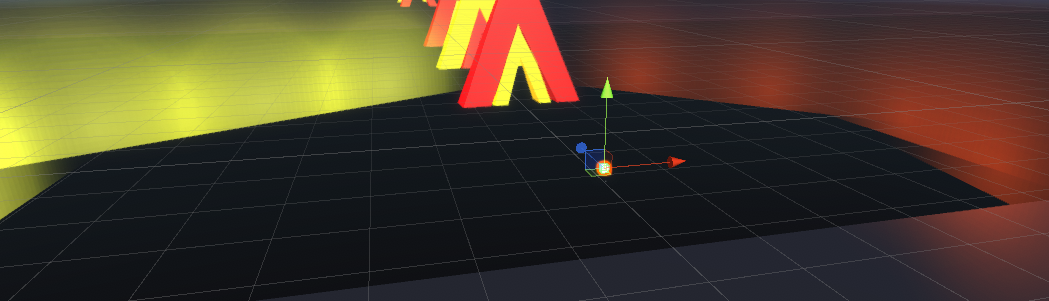
\includegraphics[width=\linewidth]{samples/image13.png}
  \caption{Triangular arcs approaching players.}
  
  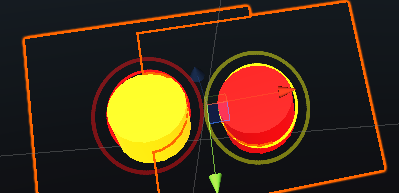
\includegraphics[width=\linewidth]{samples/image9.png}
  \caption{Coloured drums, with light response from correct note being hit}
\end{figure}

\subsubsection{Haptic}
This condition utilised the same base visuals but all audio (feedback and soundtrack) were absent. When the player hit the drums correctly they would have a high haptic feedback reward with a visual affirmation of their score going up, in addition to the lights around the "drums" lighting up and colours in the background. If the user is to hit out of time there will be no haptic response and there will be a small screen-shake, enough for the player to know they have not succeeded but to not make them feel sick.
\subsubsection{Audio}
This condition had all the same base visuals but with audio elements included, it did not reward the player with any haptic vibrations. When the player hit the drums correctly they would have a reward with a visual affirmation of their score going up, in addition to the lights around the "drums" lighting up and colours in the background. However if they were to not succeed in hitting the note, the music would drop for half a second as well as a small screen-shake would occur.

\section{Study: Haptic Vibrations as a Replacement for Audio }
\subsection{Measures}
We used one questionnaire to measure the player experience, the Player Experience Inventory (PXI) was chosen due to its ability to effectively measure the experience of the users through both their functional and psychosocial measures \cite{abeele2020development}. The PXI contains ten sub-scales within its questionnaire; Meaning, Audiovisual Appeal, Mastery, Curiosity, Immersion, Autonomy, Ease of Control, Progress Feedback, Challenge and Goals and Rule; the users were asked to rate statements in these subsections and graded them on a likert scale of 7 points. The Virtual Reality rhythm game records the player’s score. Each time a single note is hit the player will receive 10 points and they will receive 20 for every double note. This player metric was recorded to be evaluated as a measure of player performance between the two conditions. 

\subsection{Participants and Procedure}
We conducted an within-subject study with 22 participants (Average age 21.29(SD 0.96)) that were recruited through word of mouth. At the start of the study, each participant was informed on the study and provided informed consent to take part. The study was split into two conditions \textit{audio} and \textit{haptic}, order effects were controlled through a Latin Square approach. In each condition participants were asked to play each version of the condition using the Oculus Quest VR headset with each game session taken around 5 minutes. After each condition, participants were asked to fill out the questionnaire on player experience. Lastly, participants were given the opportunity to ask questions about the research and thanked for their participation. The research protocol was approved by the ethics board at removed for blind review. 

\subsection{Research Questions}
\subsubsection{Research question 1:} 
Does using haptic vibrations as a replacement for game audio affect the player experience? 
Previous literature indicates that through the use of vibrations it is possible for people to learn to play drums, or to understand their environments \cite{petry2018design}. This study seeks to find out to what extent the player experience is affected by substituting the audio in a game with haptic vibrations. We present the following hypothesis: The player experience in the \textit{haptic} condition will be worse than the \textit{audio}.

\subsubsection {Research question 2:}
Does using haptic vibrations as a replacement for game audio affect player performance? 
There is sufficient literature that states the importance of music in video games especially in rhythm games, \cite{peerdeman2010sound} indicating this would have an impact on players' competence. We present the following hypothesis: Players will perform worse in the \textit{haptic} condition than the \textit{audio}.

\section{Results}
We used using IBM SPSS v26 to compare subscales of the PXI between conditions, using Wilcoxon signed rank tests. The player metric data distribution differences were shown to be normal using the Shapiro- Wilk test of normality so we applied a paired t-test. Results are summarised in Table \ref{table:pxi}.


\begin{table}[]
\caption{Means and Standard Deviation for each dimension of the PXI split by condition.}
\label{table:pxi}
\begin{tabular}{|l|l|l|l|l|l|}
\hline
\multirow{2}{*}{Subscale} & \multicolumn{2}{|c|}{Haptic} & \multicolumn{2}{|c|}{Audio} & \multirow{2}{*}{p} \\
\cline{2-5}
& Mean & SD & Mean & SD &\\
\hline
Meaning & 4.77 & 1.52 & 4.94 & 1.23 & 0.618\\
Mastery & 4.98 & 1.35 & 4.98 & 1.10 & 0.984\\
Immersion & 4.30 & 1.63 & 5.94 & 0.98 & $<$ 0.001\\
Autonomy & 3.35 & 1.42 & 3.80 & 1.40 & 0.059 \\
Curiosity & 4.56 & 1.69 & 5.45 & 1.30 & 0.006\\
Ease of control & 5.50 & 1.31 & 5.94 & 1.08 & 0.168 \\
Challenge & 4.91 & 1.59 & 5.58 & 0.95 & 0.064\\
Progress feedback & 5.88 & 1.00 & 5.65 & 1.12 & 0.214\\
Audiovisual Appeal & 6.06 & 0.88 & 6.50 & 0.72 & 0.005\\
Goals and Rules& 6.45 & 0.68 & 6.79 & 0.38 & 0.012\\
\hline

\end{tabular}
\end{table}

\subsubsection{Player Experience}
Does using haptic vibrations as a replacement for game audio affect the player experience? Yes, the results show that the \textit{haptic} condition had several dimensions that were significantly worse than the \textit{audio} condition. \textit{The player experience in the \textit{haptic} condition will be worse than the \textit{audio}}. The results show that several dimensions of the player experience in the \textit{haptic} condition scored below the \textit{audio} condition. Statistically significant differences were found for Immersion (Z = -3.586, p $<$ 0.001), Curiosity (Z = -2.733, p = 0.006), Audiovisual Appeal (Z = -2.781, p  = 0.005), and Goals and Rules (Z = -2.514, p  = 0.012). Mean values were higher for the Audio condition in all cases.
 
\subsubsection{Performance}
Does using haptic vibrations as a replacement for game audio affect player performance? No, the results presented do not support the idea that haptic feedback as an alternative to audio has any effect on player performance. Players will perform worse in the \textit{haptic} condition than the \textit{audio}. Performance results showed no statistical difference between conditions (t=-.684, p = .501), \textit{Audio} (M=654.55, SD=144.58), \textit{haptic} (M=639.55, SD=152.21).

\section{Discussion}
Here we discuss the implications for our findings and speculate about the usage of haptic vibration feedback as an alternative to audio.

\subsection{The Importance of Audio for Immersion}
The results of the study revealed that participants felt significantly less immersed in the version that lacked audio, this echos previous findings that have highlighted how important audio in all forms is to the player experience \cite{rogers2017exploring}. When replacing audio with haptic vibrations other dimensions of the PXI were less effected, suggesting that haptic vibrations do not contribute as heavily as audio to immersion. 
\subsection{Replacing Audio}
While the findings presented point towards substituting audio feedback with haptic makes for a worse player experience. When looking at the player performance metrics we can see that no significant difference was found, indicating that both the audio and haptic feedback in isolation provided the participant with enough game information to play effectively. This could be taken further for example in situations where a game might not be able to make use of audio such as while commuting on public transport haptic feedback could be used as a replacement feedback. From an accessibility standpoint, having the auditory modality removed without choice furthers that haptic feedback could be used effectively to create a more immersive experience without cost to performance as shown by other researchers funding this idea \cite{mirzaei2020earvr}.

The absence of audio was clearly noticed by participants as reflected in the PXI, but the progress feedback dimensions was not effected, indicating that participants did not feel that they were missing game state information in either condition. 

\subsection{Why not combine them}
Since the results found a statistical difference in the PXI for half the constructs it would be interesting to look at how the two cases interacted together. So how players experience and performance would be affected when they had both audio and haptic responses. The Immersion factor was a significant difference between the cases so having them combined and compared would theoretically be increased overall for this case. The performance showed no statistical difference between the cases so if the new condition was introduced, it might be interesting to then see how participants performed.



\section{Future Work and Limitations}
There are some limitations to consider when considering the implications of our work. The testing of the hypotheses was conducted within a virtual reality rhythm game as this was the most obvious way of measuring audio against haptic responses. This limits the scope of measuring experience and performance. Using multiple games scenarios to change the genre would hopefully engage different types of players as well as give a more in depth data set to analyse for PX and performance, which is a key consideration for future work. The choice of using the PXI was determined due to its constructs covering most of what was deemed important for this project, however the use of the IGROUP questionnaire in future work would allow to understand a better understanding of how users felt present in the Virtual reality environment as it is regarded as being a key factor. The implementation of the haptic feedback was rudimentary as it simply had a binary pulse for when the user scored, future work could look at a more a complex approach to vibration as seen in recent advances through other forms such as the HD rumble from the Nintendo joy cons.

\section{Conclusion}
Previous research has highlighted on the importance of game audio has on the player experience. In our work we have found that that using haptic vibrations as a replacement to audio in a VR rhythm has a negative impact on the PX. On some dimensions this is large (Immersion) but in others the impact is quite small. While it's clear that game audio is crucial for many players, the consideration of accessibility for those with auditory impairments is apparent and needed\cite{mirzaei2020earvr}; this work therefore shows that it can potentially be replaced by haptics with only a minor compromise on player experience and no effect on performance.  






\begin{comment}
\begin{table}[]
\begin{tabular}{lllll}
\hline
                 &                     & Vrtest2 (Nohaptics) & Vrtest1(Haptics) & P values \\ \hline
PXI              & Meaning             & 4.927536232                   &    
4.826086957
              &   0.8019565147       \\ 
                 & Mastery             &  5                  &    5.028985507              &   0.9321569616       \\ 
                 & Immersion           &   5.956521739                 &   4.391304348               &  0.0003634114902        \\ 
                 & Autonomy            &   3.898550725                 &    3.434782609              &  0.141588969        \\ 
                 & Curiosity           &     5.52173913
               &   4.623188406               &  0.04975474234        \\ 
                 & Ease of Control     &  5.956521739
                  &   5.787878788               &   0.06424448719       \\ 
                 & Challenge           &    5.594202899
                &    5              &    0.1358008736      \\ 
                 & Progress Feedback   &  5.666666667                  & 5.826086957                 &  0.6105142273        \\ 
                 & Audiovisual appeal  &   6.449275362                 &   6.057971014               &  0.1418010189        \\ 
                 & Goals and Rules     &   6.724637681                 &   6.47826087               &  0.1601968918        \\ \hline
Game Scores avg. & Score               &  576.8                  &   599.2               &  0.5887385832        \\ \hline
                 & standard deviation  &     160.494542               &  142.1044542                &          \\ \hline
\end{tabular}
\end{table}
\end{comment}



%%
%% The next two lines define the bibliography style to be used, and
%% the bibliography file.
\bibliographystyle{ACM-Reference-Format}
\bibliography{sample-base}
\end{document}
\endinput
%%
%% End of file `sample-sigconf.tex'.
